\chapter{Projet : plateforme de QCM}

Le but initial du projet était de créer une plateforme en ligne proposant de remplir des QCM à des stagiaires; la plateforme étant administrable par des utilisateurs particuliers (administrateurs). Un certain nombre de fonctionnalités était attendu notamment la gestion du parcours des stagiaires, l'affichage des scores, la gestion fine des questions et réponses, etc.

\medskip

\noindent De plus, nous avons pris la liberté de rajouter des fonctionnalités :
\begin{itemize}
  \item Gestion des exceptions Java avec feedback utilisateur
  \item Gestion/vérification des \textit{input} utilisateurs
  \item Construction et définition rigoureuse de la base de données MySQL pour avoir une cohérente maximale et une redondance minimale
\end{itemize}

Par ailleurs, il était intéressant d'essayer de faire du code Java le plus réutilisable possible en utilisant notamment de l'héritage, et d'autres \textit{Design Patterns}.

\section{Choix technologiques : language, base de données, \textit{libraries}, IDE}

Comme imposé le projet a donc été fait en Java Enterprise Edition. Nous avons néanmoins souhaité utiliser \textbf{la version 8} pour pouvoir profiter des nouvelles fonctionnalités offertes sur les listes (faire un \lstinline{map} par exemple ou un \lstinline{filter}).

\medskip

À cela, s'ajoute l'utilisation de Tomcat 8 dans sa version stable. Enfin, quant à la base de données, il s'agit d'une base MySQL proposée par l'UTC sur le serveur \url{tuxa.sme.utc} (accessible uniquement sur le réseau de l'UTC) : il nous aura fallu utiliser le connecteur \lstinline{mysql-connector-java-5.1.39-bin.jar}.

\medskip

Le rendu des pages Web est fait avec JSP (JSP Standard Tag Library). Il nous aura fallu utiliser la bibliothèque \lstinline{jstl-1.2.jar}.

\medskip

Au niveau du développement, nous avons utlisé Eclipse Mars comme IDE\footnote{\textit{Integrated Development Environment}} pour sa portabilité et sa robustesse (bien que l'IDE tende de plus à plus à devenir une usine à gaz, et dont les performances sont discutables, en comparaison à d'autres IDE tels qu'IntelliJ).

\section{Rappels sur JEE}

Un bref rappel, néanmoins important, quant au fonctionnement d'une application JEE.

\medskip

Les routes sont définies dans un fichier \lstinline{web.xml}. À chaque route est associée une \textbf{\textit{servlet}}. Une \textbf{\textit{servlet}} est une classe Java particulière qui va effectuer plusieurs traitements sur deux objets particuliers (requête et réponse HTTP) avant de renvoyer une réponse au client, le plus souvent sous la forme de code HTML. Ce code HTML peut être généré à la volée ou écrit au préalable dans un fichier JSP qui sera importé. Ce fichier pré-écrit contient du code qui sera exécuté au moment de l'import, il peut s'agir de code Java ou de balises particulières JSP, mais dans les deux cas le résultat est le même.

\medskip

L'application contient également des fichiers publics, accessibles sans \textbf{\textit{servlet}}, stockés dans un sous-dossier du dossier \lstinline{WEB-INF}. Il s'agit souvent de fichier statiques tels que du CSS, JavaScript, ou des images.

\medskip

Les \textbf{\textit{servlets}} peuvent faire appel à n'importe quel autre fichier Java, instancier n'importe quels objets. C'est également ici que les appels à la base de données se font (par exemple après réception d'une requête HTTP de type POST).

\section{Architecture du projet}

\subsection{Java sources}

\begin{wrapfigure}{r}{0.25\textwidth}
  \vspace{-20pt}
  \begin{center}
    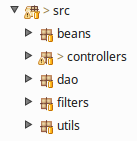
\includegraphics[width=0.23\textwidth]{images/src_archi.png}
  \end{center}
  \vspace{-10pt}
  \caption{Nos sources Java}
  \vspace{-10pt}
\end{wrapfigure}

Nous avons décidé de créer plusieurs packages, et cela dans plusieurs buts :

\begin{itemize}
    \item \textbf{beans} : Contient les classes métiers, c'est-à-dire les modèles. Il s'agit de classes simples qui sont des représentants de nos classes UML créées lors de la modélisation du projet. À chaque classe correspond une table en base de données. Ces classes contiennent les mêmes attributs que les colonnes des tables correspondantes en base de données. Les seules méthodes qui existent sont des \textit{getters/setters} et des constructeurs.
    \item \textbf{controllers} : Ce sont les \textit{servlets} qui traitent les requêtes HTTP.
    \item \textbf{dao} : Ce sont les classes qui gèrent l'accès à la base de données. Nous avons créé une classe abstraite \lstinline{DAO.java} dont toutes les classes héritent afin d'éviter autant de possible de répéter du code, notamment pour les fonctions génériques telles que \lstinline{find()}, \lstinline{insert()}, etc.
\end{itemize}

\begin{itemize}
    \item \textbf{filters} : Contient un filtre permettant d'assurer que certaines pages ne soient atteintes que par des utilisateurs connectés.
    \item \textbf{utils} : Contient des classes Java simples avec quelques fonctions \lstinline{static} afin, à nouveau, d'éviter de réécrire deux fois le même code. Ce sont des fonctions génériques utilitaires.
\end{itemize}

\subsection{WEB-INF}

\begin{wrapfigure}{L}{0.2\textwidth}
  \vspace{-20pt}
  \begin{center}
    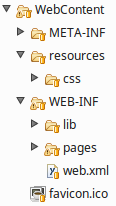
\includegraphics[width=0.18\textwidth]{images/web_archi.png}
  \end{center}
  \vspace{-10pt}
  \caption{Le dossier WebContent}
  \vspace{-2.7cm}
\end{wrapfigure}

L'autre dossier intéressant du projet est sans aucun doute \lstinline{WebContent}. Il contient beaucoup d'éléments importants répartis dans des sous-dossiers :

\begin{itemize}
    \item Les fichiers statiques servis par le serveur sur simple requête (dans notre cas, uniquement du CSS) dans le dossier \lstinline{resources}.
    \item Les 2 bibliothèques que nous utilisons mentionnées plus haut (MySQL connecteur et JSTL) dans \lstinline{WEB-INF/lib}.
    \item Les pages JSP dans \lstinline{WEB-INF/pages}.
    \item Le fichier \lstinline{web.xml} qui définit le lien entre les routes et les servlets, dans le dossier \lstinline{WEB-INF}.
\end{itemize}

\newpage

\section{Base de données}

\begin{figure}[H]
    \centering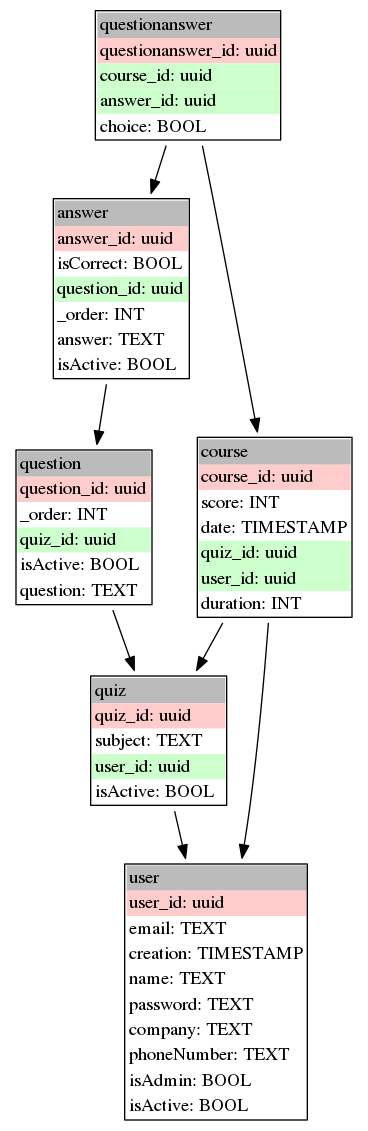
\includegraphics[width=.4\textwidth]{images/db.png}
    \caption{Schéma de notre base de données}
\end{figure}

Ce projet repose également sur l'utilisation d'une base MySQL mise à disposition par l'UTC. Cette base sert à stocker toutes nos données.

\medskip

L'une des premières étapes de ce projet, avant d'attaque tout code, a été de réfléchir à un modèle UML pour notre base de données. C'est ce même modèle qui servirait plus tard à créer nos classes métiers (\textit{beans}). Nous avons voulu éviter toute redondance (3ème forme normale). Le schéma auquel nous avons abouti se trouve sur l'image ci-dessus.

\subsection{Explications}

Ce schéma se veut le plus clair possible afin de représenter les liens qui existent entre les différentes tables. Cependant, il convient de l'expliquer un minimum et de préciser les différences avec l'implémentation réelle.

\sql
\begin{itemize}
    \item La plupart des champs sont en \lstinline{NOT NULL} par défaut sauf ceux sans importance comme l'entreprise ou le numéro de téléphone.
    \item Les clés primaires sont en \lstinline{AUTO_INCREMENT}.
    \item Les dates sont créées automatiquement grâce à \lstinline{CURRENT_TIMESTAMP}.
    \item La clé primaire de la table des utilisateurs est en fait son email (\lstinline{user_id} a été renommée en \lstinline{email}).
    \item La clé étrangère \lstinline{user_id} de la table des quizzes pointe vers le créateur du quiz.
    \item Nous avons rajouté de nombreux \lstinline{CHECK} et \lstinline{UNIQUE KEY} afin de renforcer la cohérence des données. Pour cela, voir notre fichier joint à ce rapport.
\end{itemize}

\subsection{Améliorations possibles}

\fakeshell
Le serveur ne nous permettait pas de créer de \lstinline{triggers}. C'est dommage car cela aurait pu nous permettre d'assurer une plus grande cohérence des données (par exemple vérifier qu'un créateur de quiz est administrateur, ou qu'un parcours -- \textit{course} -- est fait par un stagiaire, donc quelqu'une qui n'est pas administrateur). De même pour les colonnes \lstinline{_order}: avec des triggers nous  aurions pu les incrémenter correctement sans devoir le faire dans le code Java.

\section{Fonctionnement de l'application entière}

Comme expliqué plus haut, le fichier \lstinline{web.xml} sert à \textit{forward} la requête vers la bonne servlet en fonction du \textit{pattern} des routes. Des \textit{wildcards} peuvent être utilisés afin de \textit{match} plusieurs routes.

\medskip

La requête est ensuite envoyée soit à un filtre, soit directement à une servlet, cela dépend de ce qui est écrit dans le fichier \lstinline{web.xml}. Dans notre cas, toutes les requêtes sont transmises à un filtre, sauf une: celle à destination de la page de \textit{login}. Dans les autres cas, le filtre nous permet de nous assurer que c'est un \textbf{utilisateur connecté} qui tente d'accéder aux pages.\\
Par ailleurs, nous utilisons également un autre filtre, cette fois-ci pour \textbf{toutes les requêtes}, qui nous permet de forcer l'encodage en UTF-8. Cela est notamment très utile à la réception des requêtes de type POST. Avant cela, lorsque nous insérions des \textit{input} utilisateurs en base, le contenu reçu était implicitement converti en \textit{latin1}. Maintenant, grâce à ce filtre, il est conservé en UTF-8 et est correctement sauvegardé en base de données.

\xml
\begin{lstlisting}
<filter>
    <filter-name>Set Character Encoding</filter-name>
	<filter-class>org.apache.catalina.filters.SetCharacterEncodingFilter</filter-class>
	<init-param>
		<param-name>encoding</param-name>
		<param-value>UTF-8</param-value>
	</init-param>
	<init-param>
		<param-name>ignore</param-name>
		<param-value>false</param-value>
	</init-param>
</filter>
\end{lstlisting}

\java

À la sortie d'un filtre, la requête est transmise à une servlet. À l'éxécution de la servlet, nous avons à disposition deux objets Java (\lstinline{HttpServletRequest request, HttpServletResponse response}). Ils nous permettent respectivement de traiter la requête HTTP et la réponse HTTP que l'on enverra (accès aux \textit{headers}, au \textit{body}, paramètres GET, URL, etc.).

\begin{figure}[h]
    \centering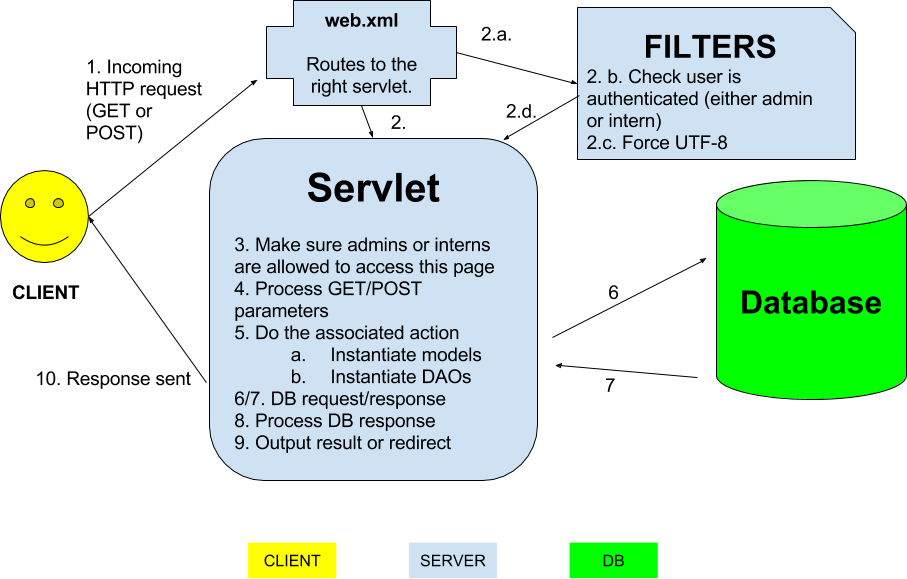
\includegraphics[width=1.00\textwidth]{images/arch.png}
    \caption{Fonctionnement de notre application}
\end{figure}

En fonction des paramètres GET (dans l'URL) ou POST (dans le \textit{body}) reçus, nous effectuons diverses opérations, souvent sur la base de données. Puis nous ``injectons'' des variables dans l'objet requête que nous ``passons'' finalement à une page JSP. Cette page va utiliser les variables injectées, qui peuvent être de type primitif, des objets, des tableaux, etc, afin d'afficher leur contenu au client.

\java
\begin{lstlisting}
public static final String REQUEST_QUESTION = "question";
...

// Injection de variables
request.setAttribute(REQUEST_QUESTION, qd.find(q));

// Appel d'une page JSP
this.getServletContext().getRequestDispatcher("/WEB-INF/pages/answersmanagement.jsp").forward(request, response);
\end{lstlisting}

\section{Implémentation}

\subsection{Servlets}

Nous avons essayé autant que possible de réutiliser les servlets plusieurs fois, afin de ne pas dupliquer du code et aussi pour simplifier notre application. Pour cela, nous avons avantageusement tiré profit de deux méthodes offertes par les servlets :

\begin{lstlisting}
@Override
public void doGet(HttpServletRequest request, HttpServletResponse response) throws ServletException, IOException {
    ...
}
@Override
public void doPost(HttpServletRequest request, HttpServletResponse response) throws ServletException, IOException {
    ...
}
\end{lstlisting}

Ces deux fonctions seront appelées en fonction du type de requête HTTP reçue : GET ou POST. Ainsi, sur plusieurs pages, notamment le login, nous pouvons utiliser la même servlet pour l'affichage du formulaire mais aussi pour la réception des identifiants de \textit{login}. Par la suite, si les identifiants sont corrects, nous redirigeons l'utilisateur, comme cela se fait sur de nombreux sites web :

\begin{lstlisting}
@Override
public void doPost(HttpServletRequest request, HttpServletResponse response) throws ServletException, IOException {
    // Vérifications des identifiants reçus auprès de la BDD

    // Sauvegarde du cookie de session
    session.setAttribute(SESSION_USER, user);
    // Redirection
    response.sendRedirect("dashboard");

    // Code ...
}
\end{lstlisting}

\subsection{Beans et DAO}

Nous avons autant de classes \textit{bean} que de DAO. La couche DAO fait office d'abstraction par rapport au modèle, afin d'effectuer des opérations en base de données.

\subsection{Filtres}

Comme dit précédemment, nous avons utilisé deux filtres dont un créé par nous. Celui-ci permet de vérifier en amont qu'un utilisateur qui tente d'accéder à une page est bien connecté (vérification des cookies). L'autre filtre permet de forcer UTF-8 sur les données reçues par l'utilisateur.

\section{Résultat final}

Ci-dessous deux extraits de deux de nos pages.

\begin{figure}[H]
    \centering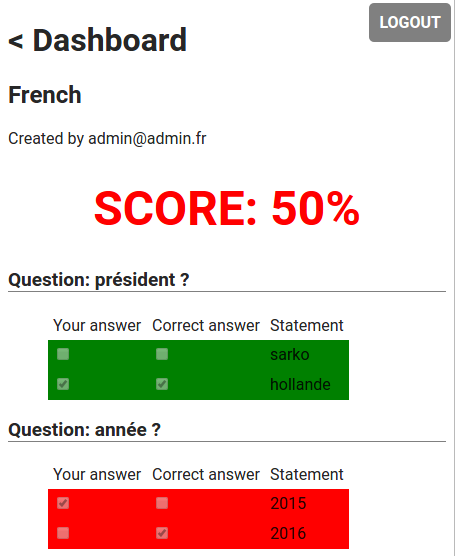
\includegraphics[width=.50\textwidth]{images/1.png}
    \caption{Fin d'un QCM}
\end{figure}

\begin{figure}[H]
    \centering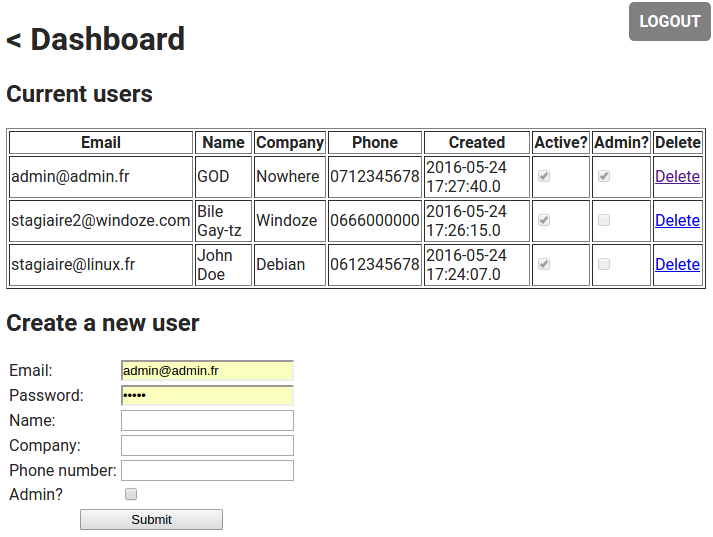
\includegraphics[width=.80\textwidth]{images/2.png}
    \caption{Liste des utilisateurs}
\end{figure}

\section{Difficultés rencontrées}

Nous n'avons pas rencontré de difficulté majeure. En revanche le projet était très chronophage et répétitif ce qui vient ternir le ressenti global.

\section{Comment exécuter le projet}

\fakeshell

\begin{enumerate}
    \item
        \begin{lstlisting}
sudo apt-get install openjdk-8-jdk
        \end{lstlisting}
    \item Télécharger \href{http://www.eclipse.org/downloads/packages/eclipse-ide-java-ee-developers/mars2}{Eclipse for Java EE} et l'installer.
    \item Télécharger \href{http://tomcat.apache.org/download-80.cgi\#8.0.35}{Tomcat 8.0.35} et extraire l'archive.
    \item Importer le projet dans Eclipse en faisant "\textit{File}" > "\textit{Import}" > "\textit{General}" > "\textit{Existing Projects into Workspace}".
    \item Corriger d'éventuels problèmes de \textit{Build path}.
    \item Installer Tomcat 8 dans Eclipse en précisant l'emplacement de Tomcat 8 qui vient d'être téléchargé et extrait.
    \item Associer le projet au serveur et lancer le projet.
    \item Puis ouvrir un navigateur Web et aller à \url{http://localhost:8080/Projet2/}.
\end{enumerate}

\section{Conclusion}

En somme, un projet très instructif et complet qui permet d'appréhender dans son ensemble la création d'une application Java EE, liée à une base de données.
